\section{CLgen: A System for Generating OpenCL Benchmarks}%
\label{sec:clgen}

This section introduces CLgen, an undirected, general-purpose program synthesizer. It adopts and augments recent advanced techniques from deep learning to learn over massive code-bases. In contrast to existing grammar and template based approaches, CLgen is entirely probabilistic. The system \emph{learns} to program using recurrent neural networks which model the semantics and usage of a huge corpus of code fragments in the target programming language.

\subsection{Overview}

Figure~\ref{fig:clgen-pipeline} provides an overview of the program synthesis and execution pipeline. CLgen learns the semantics and structure from over a million lines of hand-written code from GitHub, and synthesises programs through a process of iterative model sampling. A host driver, described in Section~\ref{sec:cldrive}, executes the synthesised programs to gather performance data for use in predictive modelling. While the approach is demonstrated using OpenCL, it is language agnostic. This approach extends the state-of-the-art by providing a general-purpose solution for benchmark synthesis, leading to better and more accurate predictive models.

Section~\ref{subsec:opencl-lang-corpus} describes the assembly of a language corpus, Section~\ref{sec:learning-opencl} describes the application of deep learning over this corpus, and Section~\ref{subsec:synthesizing-opencl} describes the process of synthesising programs.

\begin{figure}
	\centering%
	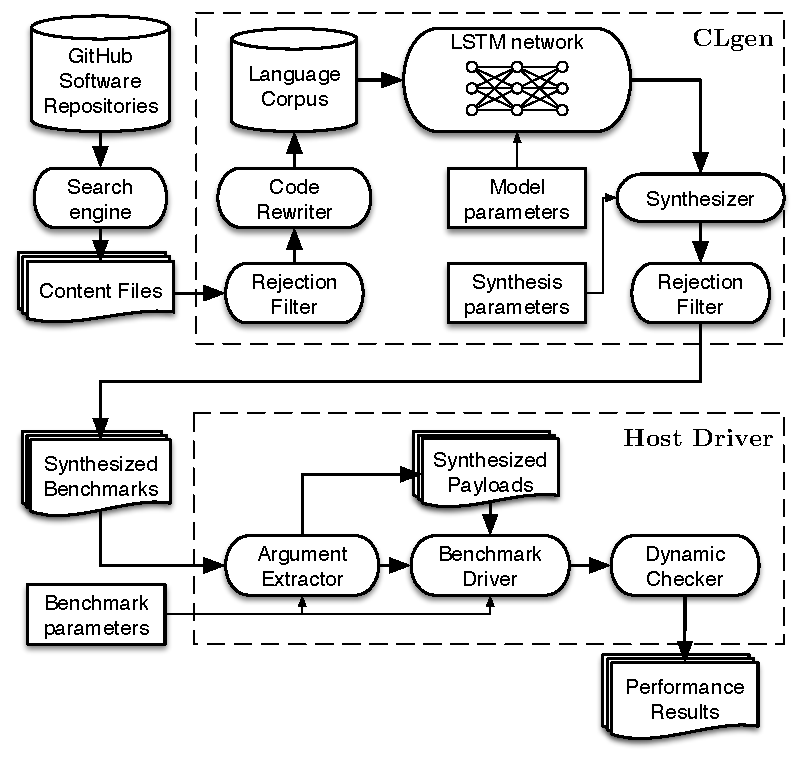
\includegraphics[width=\columnwidth]{img/pipeline}%
	\caption[Benchmark synthesis and execution pipeline]{%
    The benchmark synthesis and execution pipeline. Software is mined from GitHub; this is used to construct a language model from which new programs may be synthesised; a host driver is used to produce performance results.%
  }%
	\label{fig:clgen-pipeline}
\end{figure}

\subsection{An OpenCL Language Corpus}
\label{subsec:opencl-lang-corpus}

Deep learning requires large data sets~\cite{LeCun2015}. For the purpose of modelling a programming language, this means assembling a very large collection of real, hand-written source codes. OpenCL codes are assembled by mining public repositories on the popular code hosting site GitHub.

This is itself a challenging task since OpenCL is an embedded language, meaning device code is often difficult to untangle since GitHub does not presently recognise it as a searchable programming language. A search engine was developed which attempts to identify and download standalone OpenCL files through a process of file scraping and recursive header inlining. The result is a 2.8 million line data set of 8078 ``content files'' which potentially contain OpenCL code, originating from 793 GitHub repositories.

The raw data set extracted from GitHub is then pruned using a custom tool chain developed for rejection filtering and code rewriting, built on LLVM.


\subsubsection{Rejection Filter}
\label{subsubsec:opencl-rejection-filter}

The rejection filter accepts as input a content file and returns whether or not it contains compilable, executable OpenCL code. To achieve this, it attempts to compile the input to NVIDIA PTX byte code and performs a static analysis to ensure a minimum static instruction count of three. Any inputs which do not compile or contain fewer than three instructions are discarded.

During initial development it became apparent that isolating the OpenCL device code leads to a higher-than-expected discard rate (that is, seemingly valid OpenCL files being rejected). Through analysing 148k lines of compilation errors, a large number of failures was discovered to be caused by undeclared identifiers, a result of isolating device code. 50\% of undeclared identifier errors in the GitHub dataset were caused by only 60 unique identifiers. To address this, a \emph{shim header} was developed which contains inferred values for common type definitions (e.g. \texttt{FLOAT\_T}), and common constants (e.g. \texttt{WGSIZE}), shown in Listing~\ref{lst:opencl-shim-header}.

\lstinputlisting[%
  label={lst:opencl-shim-header},%
  float,%
  language={C},%
  caption={%
    [The \emph{shim} header file for OpenCL]An overview of the \emph{shim} header file, providing inferred type aliases and constants for OpenCL on GitHub.%
  }%
]{lst/opencl-shim-header}

Injecting the shim decreases the discard rate from 40\% to 32\%, responsible for an additional 88k lines of code in the final language corpus. The resulting data set is 2.0 million lines of compilable OpenCL source code.

\subsubsection{Code Rewriter}
\label{subsubsec:clgen-rewriter}

Programming languages have few of the issues of semantic interpretation present in natural language, though there remains many sources of variance at the syntactic level. For example, the presence and content of comments in code, and the choice of identifying names given to variables. For the purposes of generative modelling, these ambiguities are considered to be \emph{non-functional variance}. The \emph{code rewriter} is a tool developed to normalise code of these variances so as to make code more amenable to machine learning. This is a three step process:

\begin{enumerate}
  \item The source is pre-processed to remove macros, conditional compilation, and source comments.
  \item Identifiers are rewritten to have a short but unique name based on their order of appearance, using the sequential series $\{a,\allowbreak b,\allowbreak c,\allowbreak \ldots,\allowbreak aa,\allowbreak ab,\allowbreak ac,\allowbreak \ldots\}$ for variables and $\{A,\allowbreak B,\allowbreak C,\allowbreak \ldots,\allowbreak AA,\allowbreak AB,\allowbreak AC,\allowbreak \ldots\}$ for functions. This process isolates the syntactic structure of the code, and unlike prior work~\cite{Allamanis2013a}, our rewrite method preserves program behaviour. Language built-ins (e.g. \texttt{get\_global\_id}, \texttt{asin}) are not rewritten.
  \item A variant of the Google C++ code style is enforced to ensure consistent use of braces, parentheses, and white space.
\end{enumerate}

An example of the code rewriting process is shown in Listings~\ref{lst:code-rewrite-before} and~\ref{lst:code-rewrite-after}. A side effect of this process is a reduction in code size, largely due to the removal of comments and excess white space. The final language corpus contains 1.3 million lines of transformed OpenCL, consisting of 9487 kernel functions. Identifier rewriting reduces the bag-of-words vocabulary size by 84\%.

\lstinputlisting[%
  language={[OpenCL]C},%
  label={lst:code-rewriting-before},%
  float,%
  caption={[Example OpenCL content file]An example OpenCL content file downloaded from GitHub prior to code rewriting.}%
]{lst/clgen-rewrite-before}

\lstinputlisting[%
  language={[OpenCL]C},%
  label={lst:code-rewrite-after},%
  float,%
  caption={[OpenCL content file after rewriting]The example OpenCL content file of Listing~\ref{lst:code-rewriting-before} after code rewriting. Conditional compilation has been removed, the variables and functions renamed, and a code style enforced.}%
]{lst/clgen-rewrite-after}

\subsection{Learning OpenCL}
\label{sec:learning-opencl}

Generating valid, executable program code is an ambitious and challenging goal for unsupervised machine learning. CLgen employs state-of-the-art deep language modelling techniques to achieve this task.

The Long Short-Term Memory (LSTM) architecture of Recurrent Neural Network~\cite{Sundermeyer2012,Mikolov2015} is used to learn a character-level language model over the corpus of OpenCL compute kernels. The LSTM network architecture comprises recurrent layers of \emph{memory cells}, each consisting of an input, output, and forget gate, and an output layer providing normalised probability values from a 1-of-K coded vocabulary~\cite{Graves}.

A 3-layer LSTM network is used with 2048 nodes per layer, implemented in Torch. This 17-million parameter model is trained using \textit{Stochastic Gradient Descent} for 50 epochs, using an initial learning rate of 0.002, decaying by a factor of one half every 5 epochs. Training took three weeks on a single machine using an NVIDIA GTX Titan, with a final model size of 648MB. Training the network is a one-off cost, and can be parallelised across devices. The trained network can be deployed to lower-compute machines for use.

\subsection{Synthesising Source Code}
\label{subsec:synthesizing-opencl}

OpenCL compute kernels are synthesised by iteratively sampling the learned language model. Two modes for model sampling are supported: the first involves providing an \emph{argument specification}, stating the data types and modifiers of all kernel arguments. When an argument specification is provided, the model synthesises kernels matching this signature. In the second sampling mode this argument specification is omitted, allowing the model to synthesise compute kernels of arbitrary signatures, dictated by the distribution of argument types within the language corpus.

In either mode a \emph{seed} text is generated and model is sampled, character by character, until the end of the compute kernel is reached, or until a predetermined maximum number of characters is reached. Algorithm~\ref{alg:clgen-synthesis} illustrates this process. The same rejection filter described in Section~\ref{subsubsec:opencl-rejection-filter} then either accepts or rejects the sample as a candidate synthetic benchmark. Listings~\ref{lst:clgen-sample-a},~\ref{lst:clgen-sample-b}, and~\ref{lst:clgen-sample-c} show three examples of unique compute kernels generated in this manner from an argument specification of three single-precision floating-point arrays and a read-only signed integer. The quality of synthesised code is evaluated in Section~\ref{sec:clgen-qualitative-evaluation}.

\begin{algorithm}
\begin{algorithmic}[1]
\Require LSTM model $M$, maximum kernel length $n$.
\Ensure Completed sample string $S$.
\State $S \gets$``\texttt{\_\_kernel void A(const int a) \{}''\algorithmiccomment{Seed text from argument specification}
\State $d \gets 1$\algorithmiccomment{Initial code block depth}
\For{$i \gets |S|$ \textbf{to} $n$}
  \State $c \gets PredictCharacter(M, S)$\algorithmiccomment{Generate new character}
  \If{$c = $``\texttt{\{}''}
    \State $d \gets d+1$\algorithmiccomment{Entered code block, increase depth}
  \ElsIf{$c = $``\texttt{\}}''}
    \State $d \gets d-1$\algorithmiccomment{Exited code block, decrease depth}
  \EndIf
  \State $S \gets S + c$\algorithmiccomment{Append new character to sample}
  \If{$depth = 0$}
    \State \textbf{break}\algorithmiccomment{Exited function block, stop sampling}
  \EndIf

\EndFor
\end{algorithmic}

\caption[Sampling a candidate kernel from a seed text]{Sampling a candidate kernel from a seed text.}
\label{alg:clgen-synthesis}
\end{algorithm}

\lstinputlisting[%
  float,%
  label={lst:clgen-sample-a},%
  caption={%
    [Synthesised vector operation with branching and synchronisation]%
    CLgen-synthesised vector operation with branching and synchronisation.%
  },%
	language={[OpenCL]C}%
]{lst/clgen-sample-a}

\lstinputlisting[%
  float,%
  label={lst:clgen-sample-b},%
  caption={%
    [Synthesised zip operation]%
    CLgen-synthesised zip operation which computes $c_i = 3a_i + 2b_i + 4$.%
  },%
  language={[OpenCL]C}%
]{lst/clgen-sample-b}

\lstinputlisting[%
  float,%
  label={lst:clgen-sample-c},%
  caption={%
    [Synthesised partial reduction operation]%
    CLgen-synthesised partial reduction over reinterpreted vector type.%
  },%
  language={[OpenCL]C}%
]{lst/clgen-sample-c}
